\documentclass[10pt,a4j,twocolumn]{jsarticle}

\usepackage[dvipdfmx]{graphicx}
\usepackage{url}
\setlength{\textheight}{275mm}
\headheight 5mm
\topmargin -30mm
\textwidth 185mm
\oddsidemargin -15mm
\evensidemargin -15mm
\pagestyle{empty}
\begin{document}
\title{ユーザメモとwikiを連携するシステムの開発}
\author{関西学院大学理工学部 情報科学科 西谷研究室 3550 江本沙紀}
\date{}
\maketitle
\section{開発の背景}
近年,ナレッジマネジメントが企業経営の重要な要素と言われ,
導入を進める企業が増えている.
ネレッジマネジメントとは,個人の持つ知識や情報を組織全体で共有し,
有効に活用することで実績を上げようという経営手法である.

ナレッジマネジメントでは,グループ開発において共有する知識は暗黙知と形式知に分けられる[1].
暗黙知は主に口伝によって一対一でつたえられたり,あるいは体で覚えるというのが一般的である.
しかし,定着するまでの間は一般的にメモという形で個人的な知識として扱われるのが普通である.
一方,形式知は図書館やweb上に誰もが読める形で保管,提供される.

西谷研究室では,各所属学生の暗黙知を形式化するために,my\_helpというgemを開発し,
自分のためのメモをのこして活用している.本研究では,西谷研究室内でのナレッジマネジメントを
推進するため,my\_helpからwiki cloneのhikiへ自動変換するシステムの開発と,
my\_helpをよりよいソフトにするためにFrontPageの設計をする.

\section{開発の方法}
想定しているこのシステムの使用法は以下の通りである.

\begin{enumerate}
\item my\_helpを利用してメモを作成する.
\item 研究室内の各学生のメモを1つの場所に集めるためにサーバに送る.
\item サーバに集めたメモをhiki形式に変換して,wikiで表示する.
\item 研究室に所属するメンバーが全員のメモを閲覧し情報を共有する.
\end{enumerate}
このような動作をすることのできるコマンドの開発を行う.

\section{結果}
コマンドを2つに分けてシステムの開発を行った.

\begin{itemize}
\item TARGET --push
\end{itemize}
\begin{description}
\item my\_helpで作成したメモが自動的に保存される.my\_helpのディレクトリから,
必要なメモのみを西谷研究室で使用しているサーバであるnishitani0
にscpコマンドを利用してコピーする.
同時にコピーができているかの確認も,
コマンドによって行うことができるような仕様になっている.
\end{description}
\begin{itemize}
\item my\_help --hiki 
\end{itemize}
\begin{description}
\item 作成したメモをhikiの形式に変換し,wikiで表示することのできる
/Sites/hiki-1.0/data/textにコピーする.
全てのメモへのリンクがあるトップページであるFrontpageを作り,
自動で表示を行う.
\end{description}

\section{FrontPageの設計}
知識共有のため,以下のような機能の実装を設計した.

\begin{itemize}
\item メモの内容による分類
\item 研究室内のメンバーのhelpへのリンク
\item 閲覧回数が上位のhelp
\item 更新の新しいhelpへのリンク
\item pdf形式に変換し印刷
\item 分類内で閲覧回数の多いhelpへのリンク
\end{itemize}

\begin{figure}[htbp]
\begin{center}
\begin{tabular}{c}
\begin{minipage}{0.5\hsize}
\begin{center}
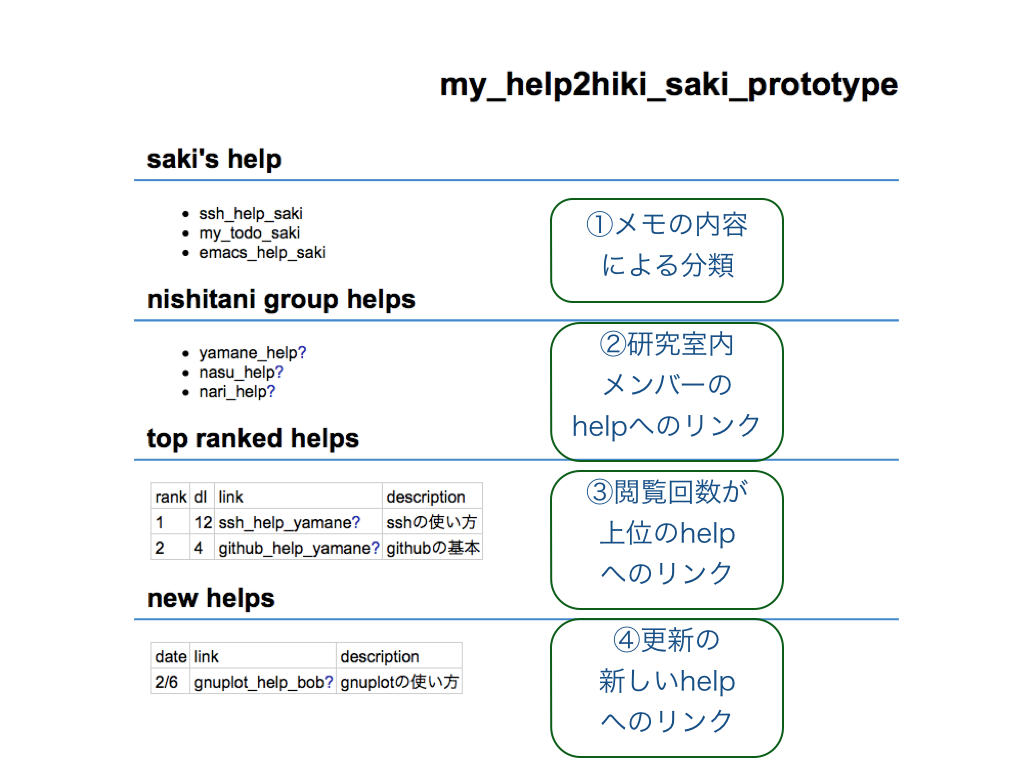
\includegraphics[width=4.5cm,bb=100 100 1000 1000]{my_help2hiki_saki.014.png}
\end{center}
\hspace{1cm} FrontPage

\end{minipage}
\begin{minipage}{0.5\hsize}
\begin{center}
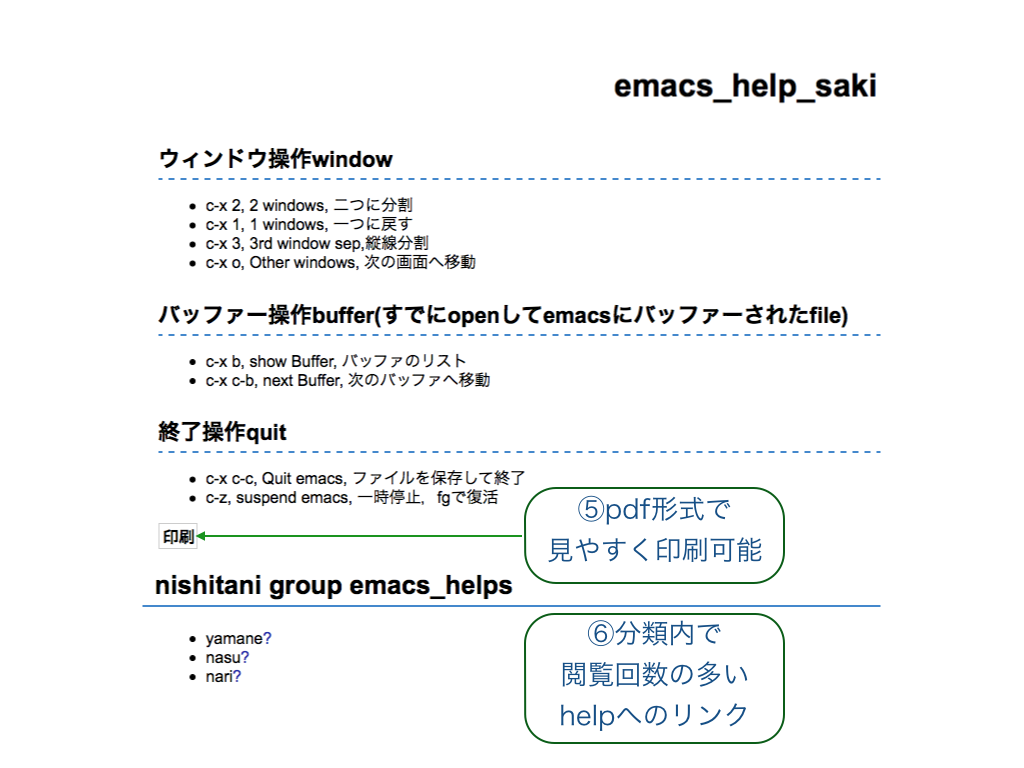
\includegraphics[width=4.5cm,bb=100 100 1000 1000]{my_help2hiki_saki.015.png}
\end{center}
\hspace{1cm} (例)emacs\_help

\end{minipage}
\end{tabular}
\end{center}
\end{figure}

\section{今後の課題}
西谷研究室には内部サイトがあり,研究室内で使用するシステムのマニュアル等が公開されている.
本研究で表示を可能にしたFrontPageを内部サイトに表示するようにすれば,
さらに研究室内のナレッジマネジメントに役立つのではないかと考えている.
今後,作成したFrontPageの設計に従い開発を続けてほしい.

\section{参考文献}
[1]ニック・ミルトン,「プロジェクト・ナレッジ・マネジメント」,
(生産性出版,東京都渋谷区渋谷3-1-1,2009年),p.4-5
\end{document}
